\documentclass[a4paper]{article}
%\usepackage[parfill]{parskip} 
\usepackage[T1]{fontenc}
\usepackage{a4wide}
\usepackage[utf8]{inputenc}
\usepackage[usenames,dvipsnames]{color}
\usepackage{graphicx,float,wrapfig}
\usepackage{listings}
\usepackage{caption}
\usepackage{subfig}
\usepackage{url}
\usepackage[left=2.5cm,top=3.5cm,right=2.5cm,bottom=3cm]{geometry}

\definecolor{MyDarkGreen}{rgb}{0.0,0.4,0.0}
\lstset{
        basicstyle=\small\ttfamily,
        keywordstyle=[1]\color{Red}\bf,
        keywordstyle=[2]\color{Purple},
        keywordstyle=[3]\color{Blue}\underbar,
        identifierstyle=,
        commentstyle=\usefont{T1}{pcr}{m}{sl}\color{MyDarkGreen}\small,
        stringstyle=\color{Purple},
        showstringspaces=false,
        tabsize=4,
        frame = ,
        morekeywords={result, action, do, data, extern, request, class, new, module,import,where,let,case,if,then,else,elsif,forall, struct},
        morekeywords=[2]{},
        morekeywords=[3]{},
        morecomment=[l][\color{Blue}]{...}
        }

\newcommand{\timbercode}[2]
  {\begin{itemize}\item[]\lstinputlisting[caption=#2,label=#1]{#1.t}\end{itemize}}

\makeatletter
\renewcommand\paragraph{\@startsection{paragraph}{4}{\z@}%
  {-3.25ex\@plus -1ex \@minus -.2ex}%
  {1.5ex \@plus .2ex}%
  {\normalfont\small\bfseries}}
\makeatother

\begin{document}
\title{ Designing a Timber Interface to the Cocoa Framework}
\author {Daniel \"{O}hrlund and Victor Danell}
\date{\today}
\maketitle
\thispagestyle{empty}

\begin{abstract}
The main goal in this project was to design the architecture of a Timber interface to the Cocoa/ Objective-C programming environment. With Timber and Cocoa using different run-time systems, it was important to determine what requirements the design had to fulfill, in order for the two systems to cooperate successfully. Memory management and threading were the main areas where decisions had to be made that greatly influenced the design of the interface.

The resulting interface implementation leverages the strengths of Timber and Objective-C, and is both robust and easy to use. As there are two run-time systems running concurrently, some extra overhead is to be expected, but testing has shown the decrease in performance to be negligible in cases of normal use.
\end{abstract}

\newpage
\tableofcontents

\newpage
\section{Introduction}
Adding a graphical user interface (GUI) to an application makes it easier to use and to interact with. The Timber programming language \cite{timberLang} would benefit from allowing access to a GUI framework, as developers could then present their applications in a more user-friendly manner.

Apple's Cocoa framework \cite{cocoaLib} is the most commonly used GUI framework on Mac OS X, but despite being very popular, it can be improved upon; for example, it relies at times on informal requirements specified only in the documentation, leaving programmers at risk of writing code that does not behave as expected.

The main goal of this project was to design the architecture of a Timber interface for the Cocoa framework to enable construction of GUI applications for the Mac OS X platform using Timber. Features of the Timber language were leveraged to present a more uniform and robust interface to  Cocoa. For example, Timber's type system helps ensure that the informal requirements specified by Apple are met, allowing mistakes previously not discovered until run-time to no longer make it past compilation. The goal was to make the right way to code the only way to code.

\section{Background}
\subsection{Timber}
Timber is a strongly-typed, functional, object-oriented language with object-level concurrency \cite{timberLang}. Functions in Timber are stateless blocks of code that perform calculations when executed and the result from invoking a function depends only on the values of its parameters; calling a function will not cause side-effects. Objects in Timber contain methods and state variables, where the state variables of an object are only reachable from within its own methods.

There are two types of methods in Timber: requests and actions. Both of these types execute one or more commands in sequence when invoked, and calling a method may produce side-effects. Different types of methods infer different synchronization: on a request, the caller will wait until the method execution has finished and on an action, the caller will wait until method execution has started. There is also a way to bypass synchronization altogether (and even to delay an activation of the action) by prefixing the method call with the keyword \textit{send} (with an \textit{after [time]} construction if necessary).

\subsubsection*{Execution model}
Timber has a reactive execution model, where method invocations are triggered by messages sent either from other methods, or from the environment.

\subsubsection*{Concurrency model}
Timber offers an implicit concurrency model with object-level concurrency, which means that methods belonging to different objects may execute concurrently. To prevent race conditions in the state of an object, only one method of the object may be active at any given time. 

\subsubsection*{Types, objects and sub-typing}
Timber is a strongly-typed programming language that supports declarative sub-typing and parametric polymorphism for record types, as well as declarative super-typing for data types. Objects are created using classes but there is no inheritance in Timber. 

The \textit{class} keyword in Timber is used to create a class definition that may contain methods and state variables, and must return a value. The returned value is the only means of interaction with an object of that class and is commonly referred to as the \textit{interface} of the object.

Objects in Timber can be constructed in hierarchies, with an object made up entirely, or in part, of other objects. This means that the interface returned by the invocation of a new statement may contain values (typically -- methods) from multiple objects.

\subsubsection*{Mutable and immutable data}
State variables of objects are the only mutable data in Timber (a state variable of an array type can be updated as a whole or only partially), whereas records, lists, arrays, etc. that are not state variables are immutable.

\subsubsection*{External functions}
Native functions (written in C for the POSIX platform and in JavaScript for the Browser platform) can be accessed from within Timber code by declaring their type signature at the top level of a module, prefixed with the keyword \textit{extern}. If a module M refers to an external function in this manner, the corresponding C code and header files should be M.extern.c and M.extern.h, respectively.

\subsection{Timber's rtsPOSIX}
The Timber run-time system used in this project is rtsPOSIX, a run-time system that makes use of the POSIX API, including POSIX threads (pthreads) and UNIX signals. The Timber module POSIX  allows applications to interact with the POSIX environment.

\subsubsection*{Garbage collection}
Garbage collection in rtsPOSIX is performed automatically by an incremental, copying garbage collector (GC)  \cite{kero1, kero2}. During a GC pass, the GC scans the heap for objects that are reachable from a set of root nodes and copies them to the new heap. Data not reachable from any root node is not copied.

When external functions are involved, an object referenced from the external code must be preserved during garbage collection even if it is not reachable from any root node in Timber. The C function \textit{addRootScanner} in rtsPOSIX registers a custom function to be run during garbage collection, and can be used for ensuring that such objects are copied to the new heap.

\subsection{Objective-C run-time and the Cocoa framework}
Objective-C is a programming language that extends the standard ANSI C language with object-oriented capabilities. In Objective-C, decisions are made at run-time when possible, rather than at compile-time. The API of the Objective-C run-time used on the Mac OS X platform is unique to that platform \cite{objcRuntime}.

The Cocoa API  \cite{cocoaLib}  is a set of frameworks developed by Apple that together make up a programming environment for Mac OS X and iOS operating systems. Cocoa applications usually follow Apple's Human Interface Guidelines \cite{cocoaGuidelines}.

\subsubsection*{Memory management in Objective-C}

Objective-C supports three memory models: manual reference counting, automatic reference counting and automatic garbage collection.

\subsubsection*{Reference counting}
NSObject is the root class of most Objective-C class hierarchies. Through NSObject, objects inherit a basic interface to the run-time system and the ability to behave as Objective-C objects. Every NSObject has its own \textit{retain count},  which upon object creation (or copying) is set to one. After an object has been created, other objects may want to ``own'' the object; this is done by \textit{retaining} the object, which increases its retain count by 1. Owners of an object may also give up their ownership by \textit{releasing} the object, which decreases its retain count by 1. If a release sent to an object causes its reference count to reach 0, the object will be deallocated \cite{cocoaMemory}.

Cocoa also allows for objects to be \textit{autoreleased}, which means that the object is placed in an autorelease pool that, once the pool is drained, will release the object. More than one reference to an object can exist in an autorelease pool at once and each reference will trigger sending of a release message to the object (in other words, an object added to the same autorelease pool twice will upon a pool drain receive two release messages). This is safe even though an object may have deallocated itself (if its retain count hits 0), since passing a message to \textit{nil} will not do anything.

An autorelease pool belongs to a particular thread, and pools for each thread are arranged in a stack. When  automatic reference counting is not used, Cocoa expects that an autorelease pool is always available, which leaves it up to the programmer to ensure the existence of such a pool when working with multiple threads. Since Cocoa automatically creates an autorelease pool at the beginning of each iteration of the main event loop, the programmer does not need to create them unless other threads are created. A local autorelease pool can also be used to reduce the peak of the memory footprint, in sections where many temporary objects are allocated.
\\ \\ \textit{Manual reference counting} \\
When using manual reference counting, the programmer has to take care of all retain and release messages.
\\ \\ \textit{Automatic reference counting (ARC)} \\ ARC is a technique implemented in the LLVM compiler \cite{llvmARC} that performs static analysis of program code during compilation and inserts code sending retain and release messages automatically.
\\ \\ \textit{Automatic garbage collection} \\ When automatic garbage collection is enabled, instead of using the regular retain count of objects to determine when an object should be deallocated, the garbage collector analyzes the heap to find all reachable objects from a set of well-known \textit{root objects}. The collector  follows all strong references from the root objects and its children until there are no more references to follow, and the objects that have not been added to the set of reachable objects are \textit{finalized} (NSObject implements a method \textit{finalize}) and the memory is released.

\subsubsection*{Concurrency model in Objective-C}
Two types of threads are supported by the Objective-C run-time: NSThreads and POSIX threads (pthreads). Although these can be used directly, starting in Mac OS X 10.6 the \textit{libdispatch} library introduces a feature called \textit{Grand Central Dispatch} (GCD) that not only abstracts away the work of spawning and keeping track of new threads, but also helps balance load between CPU cores \cite{cocoaGCD}.

The two basic functions of GCD are \textit{dispatch\_async} and \textit{dispatch\_sync}, and they send blocks of code to queues; a queue has a list of blocks to invoke and it is typically not known on which thread a queue will execute, except in the case of the queue returned by the function \textit{dispatch\_get\_main\_queue()} (which will execute on the main thread, interleaving with processing GUI events in GUI-enabled applications). Internally, GCD keeps a pool of threads to run code on, from which queues check-out threads to use. When a queue has finished executing, it will return the thread to the pool.

\subsubsection*{Cocoa's thread requirements}
Cocoa contains many classes that are considered thread-safe, but also some that are declared unsafe. Thread-safe classes can be used from multiple threads simultaneously, whereas the behavior of unsafe classes in such cases is undefined. Documentation released by Apple states that ``in most cases, you can use these classes from any thread as long as you use them from only one thread at a time''.

In addition to the above, there are also main-thread-only classes, instances of which are intended to be used exclusively on the main thread of an application. Generally when constructing GUI applications, classes of all three types are used. NSWindow is an example of a commonly used thread-unsafe class, while NSView together with all of its descendants are main-thread-only classes (which pretty much includes every GUI object since NSView is the basic class for something that is viewable). 

Cocoa requires that the main event loop of an NSApplication be executed on the main thread of a process (thread 0). The main event loop is responsible for reading and dispatching events, and having all events processed on the same thread prevents them from appearing out of sequence. Dispatch queues can be used to ensure code is executed on the main thread, either synchronously with dispatch\_sync or asynchronously with \textit{dispatch\_async}, by dispatching to the queue returned by  \textit{dispatch\_get\_main\_queue} \cite{gcdMainQueue}.

\subsubsection*{Inheritance and delegates}
Although sub-classing is often used in Cocoa, extending the functionality of a class is a task generally performed by \textit{delegates}. Delegates are loosely coupled to the class with which they are used, and are often specialized to perform particular tasks.

\subsubsection*{Event handling}
There are a lot of different types of events in Cocoa, for example: key pressed events, key released events and left mouse button clicks. Events are delivered to the main event loop, where they are placed in a FIFO queue. The main event loop continuously gets the topmost event, converts it to an NSEvent and dispatches it to its final destination.

The destination of an event depends on its type; mouse events are sent to the window in which the event occurred (the window that the mouse cursor was placed in), while key events take a different route which includes key equivalents (global shortcuts for an application such as CMD+W for closing a window) and key interface controls (key presses that should control the interface, such as Tab that shifts focus), but ultimately they reach the component that is currently in focus. 

\section{Design Choices}
When designing the Timber interface to Cocoa, care has been taken to minimize the risk of mistakes that can be made by a programmer using the interface, while keeping as much flexibility as possible.  Mistakes related to threading have been completely eliminated, and the stronger type system of Timber has removed the risk of run-time exceptions from objects in Cocoa being passed messages to which they cannot respond (with the usual reservation as to possible errors in our implementation).

\subsection{Combining the two run-time systems}
As seen earlier, the two run-time systems have different views on concurrency. To be able to combine the two, we have to meet Cocoa's special requirements regarding the use of the main thread without breaking Timbers implicit threading model.

We thought about implementing a custom RTS for this purpose, but decided to leave that idea and stick to using rtsPOSIX with as few modifications as possible. This decision was made to keep the maintenance cost of Timber run-times low, and also to be able to benefit from future improvements of rtsPOSIX.

Since Cocoa has support for multi-threading and pthreads, rtsPOSIX can be used with a few changes: we needed a way to claim the main thread and dedicate it to Cocoa, and a way to guarantee that classes that are main-thread-only are executed on the main thread. We implemented a small modification in rtsPOSIX which, after the RTS has been initialized, enables execution of a callback method (installed dynamically by the application) on the main thread (later on, this feature was incorporated in the ``default'' rtsPOSIX). Methods of Timber objects can be executed on any of the worker threads, so we are using GCD to dispatch all work that requires main thread execution to the main queue that, according to Apple's documentation, runs on the main thread \cite{gcdMainQueue}.

Another important decision regarding the two run-time systems is how to manage memory in Objective-C. As discussed earlier, there are three possible alternatives: manual reference counting, automatic reference counting, and automatic garbage collection. Automatic reference counting was not an option in this project since does not allow storing object pointers in C structures \cite{arcIOS}, which is something we have to do frequently. Choosing between manual reference counting and automatic garbage collection we picked manual reference counting, both due to the fact that it performs better given that we write correct code, and because automatic GC is not supported in iOS. Even though the scope of this project does not include iOS, it has been considered as a possible future implementation and choosing manual reference counting prepares us well for that.

\subsection{Two-part objects}
Timber and Cocoa each have their own heaps and garbage collectors (GCs). The GUI objects designed in this project consist of data stored in both heaps, and are referred to as \textit{two-part} objects. The Timber side of a two-part object includes a value of the CocoaRef type (an abstract type synonymous to Int) that is a unique reference to the corresponding Cocoa object. Values of this type are never constructed in Timber but are returned by external methods, which take an argument of type World. External methods that propagate changes in Timber to Cocoa all require an argument of type CocoaRef.

To implement our design of two-part objects in a simple way, we introduced the concept of \textit{component state} for the Timber part of such an object. A GUI component can be in one of three different states: \textit{Active}, \textit{Inactive} or \textit{Destroyed}. When the object is first created, it will be in the Inactive state, and it will only be allocated on the Timber heap. Modifying the object will not make any callbacks to its Cocoa counterpart (since there is none), but only update the Timber object.

When an object changes its state to Active, the corresponding Cocoa part will be allocated and a reference to it will be stored in the Timber object to be able to perform callbacks when the object is modified. For regular components, this state change will either happen when the object is added to an initialized window or container (i.e., one in the Active state), or when the object is already added to a container or a window and the window or the container is initialized.

\subsection{Collaboration between Timber's and Cocoa's garbage collectors}
Whenever a Timber object is garbage collected, the corresponding object data on the Cocoa heap should be released as well. However, since Timber does not have an equivalent of Java's \textit{finalize()} methods \cite{javaFinalize},  Timber's GC cannot release Cocoa objects. Modifying the GC to enable this is possible, but is a change that would introduce other issues, such as potentially decreased performance and difficulties in maintaining the code for the GC. Instead, our solution is to postpone allocation of the Cocoa part of an object until initialization, which occurs when the Timber object is added to an initialized container or window; a window and all its children are initialized when it is added to a Cocoa application. At the same time, the Cocoa part of the object is deallocated when the Timber object is destroyed, which occurs when it is removed from its parent or when the window is destroyed. Windows are considered to be external resources that need to be destroyed explicitly.

A second issue relating to the GC is that of updating references between heaps. It was initially believed that the Timber and the Cocoa halves of a component would each require a reference to the other half, which proved complicated as Timber divides its heap into two parts, copying objects between them during garbage collection. Pointers from the Cocoa heap would have to be updated whenever the GC in Timber is run. Given the frequency of scans and the possibly large number of components present in an application, this could have a negative impact on performance. However, it was discovered that Cocoa objects do not need to know about their corresponding Timber half (see the section on event dispatching below); all they need is a reference to the  \textit{Cocoa application}. This can be solved by using a custom root scanner registered with rtsPOSIX so that the reference to the Cocoa application is updated during each GC pass in Timber (see the section on implementation of event handling for more details). Any notifications received in Cocoa, which Timber needs to be informed of, can simply be passed to methods of the application that will then deal with dispatching them to the correct destination in Timber.

\subsection{Event dispatching}
Cocoa events are delivered to objects in Cocoa automatically but it is up to us to make sure they reach their corresponding Timber component. As discussed in the previous section, keeping a reference in a Cocoa object to its Timber counterpart is difficult at best, which means we will not be able to pass events directly between objects.

To solve this issue, an important realization is that an object can only receive events if it is contained in a window. Since we can ``hijack'' events in Cocoa on their way to a window, and pass them to their corresponding CocoaWindow in Timber, we can \textit{reproduce the event dispatching in Timber} and deliver each event to its respective component ourselves, without Cocoa having to know about any Timber object apart from the application.

With windows in Cocoa all having unique IDs, the \textit{initWindow} method of CocoaWindow returns a value of type \textit{WindowID} (which is an abstract type synonymous to Int) alongside its \textit{CocoaRef} value; this value is then used to identify the window that should receive a certain event. 

As a consequence of this decision, we have to maintain our own focus hierarchy in Timber in order to dispatch key events, since we will not be able to use Cocoa's focus hierarchy.

\subsection{Cocoa-specific types}
When changing the properties of GUI objects in Cocoa, one has to use Cocoa specific types, such as NSString for titles and CGRect for rectangles. Considering the fact that Timber already has its own versions of many of these types, exposing access to the Cocoa types would serve no purpose and would only be confusing. Therefore, the interface accepts Timber types, which are translated into the corresponding Cocoa types as necessary.

\section{The Solution}
When designing the application interface, we had two options: we could either design a general interface that contained methods for starting an application, adding a new window to the application, setting up application preferences such as name, icon and the menu bar, etc.; or we could divide the interface into two parts, where the first part would represent the ``OS layer'', used only to configure (set up preferences) and start an application, and the second part would represent the actual application, with methods that can make windows visible in the application, etc.

We decided to go with the latter, for many reasons. For example, it allows us to ``hide'' things from the general interface that can not actually be done until the application has started, such as making a window visible, thereby making the resulting interface easier to understand. The type of the general interface is \textit{CocoaEnv}, and the \textit{App} is the the type of the interface of a running application.

\subsection{The Cocoa environment}
The CocoaEnv type (shown in Listing \ref{cocoaEnv})  allows us to initialize a Cocoa application, using the \textit{startApplication} method. In order to ensure a Cocoa method is always executed within the scope of a valid application, \textit{startApplication} takes an (App --> Action) callback that is to contain all code dependent on the App object. This precludes undefined behavior in a multi-threaded setting.
The callback is invoked when the application is ready to be used; that is, when the created NSApplication receives its \textit{didFinishLaunching} notification.

The environment class \textit{cocoa} is defined externally for two reasons. The first one is that the created object is a singleton, and to prevent instantiation of more than one object we have defined the class so that the first call to \textit{cocoa} will create an object and return its interface (of type CocoaEnv), and all subsequent calls will return the same interface. The second reason is that since the only method in the class definition is \textit{startApplication}, which is responsible for initializing Cocoa, all code in \textit{startApplication} has to be defined externally anyway.

The external class \textit{cocoa} takes an argument of type World. This is a semantic dependency, meant to clarify that there are external dependencies not directly exposed by the environment. In a sense, the World is the environment in which the Cocoa application exists.

\timbercode{cocoaEnv}{"CocoaEnv"}

\subsection{The application}
An object of type App (i.e, an object with the interface of type App, which is shown in Listing \ref{app}) is used for communication from Timber to an already initialized NSApplication in Cocoa. The class \textit{cocoaApplication} in COCOA.t is not intended to be used by programmers directly, but is rather the class definition used by the environment to instantiate the application object returned to the callback of \textit{startApplication}.

The method \textit{addWindow} will initialize a CocoaWindow, thereby making it appear on screen. It will also store a reference to the window in a list, so that it will not be garbage-collected until it is (eventually) destroyed.

The three methods \textit{sendInputEvent}, \textit{sendWindowResize} and \textit{sendWindowCloseRequest} will be invoked by messages sent from the environment when external events are received. They are separated from \textit{addWindow} to make it clear that they are not intended to be called by the programmer.

\timbercode{app}{"App"}

\subsection{GUI components as two-part objects}
In order to access the Cocoa part of an object, it is clear that there will have to exist external methods in Timber. Not as clear, however, is where to draw the line when a method should be made external. To keep readability, maintainability, and type safety to a maximum, it was decided to keep all component classes written mainly in Timber, with only the bare minimum of functionality delegated to external methods. There is a slight trade-off in performance, as a number of conversions between Timber and C types are required, but the gains far outweigh this minor cost.

The state of a component is kept in both Timber and Cocoa. This choice was made to support uninitialized components as Timber objects with modifiable properties, which would not have been possible with the state only kept in Cocoa. However, text components are currently treated differently: instead of replicating Cocoa's handling of text input (e.g., deleting marked text and keeping track of  the cursor's position), which would have been very complicated, the text content is kept in Cocoa only and retrieved by Timber on demand. Worth noting is that each text object will also have a text state variable to support uninitialized text components.

\subsection{Initialization and memory management}
All component types have methods \textit{initComp} and \textit{destroyComp}  that are used for initializing and destroying objects, respectively. The \textit{initComp} method sets a component's state to Active, initializes it in Cocoa and matches the parameters of the Cocoa object to the component properties in Timber; it also updates the component's CocoaRef value to the memory address of the created Cocoa object. This method is called automatically when a component is added to an active component (e.g., an active window or a container inside an active window). 

These methods are not intended to be used directly by a programmer of a GUI application. Instead, they will be triggered on a component when it is either added to an already active container or a window, or when its parent component is made active, which happens, for example, when a window is added to an App. Components expose these methods to allow parents to initialize and destroy them without having to know their exact type. To release memory for a component while its parent is still active, the component has to be removed using the parent's \textit{removeComponent} method.

If a new container class is implemented, the \textit{initComp} should be called on all added components as appropriate. There must also be an application available before objects are allocated in Cocoa and therefore \textit{initComp} takes  an App as its first argument; this prevents allocations of GUI components before the Objective-C run-time has been properly initialized.  It is also important to call the added component's \textit{destroyComp} method when the container is destroyed or the component is removed, for the allocated memory to be released in Cocoa. 

When a window is initialized by the method \textit{addWindow} of an App, it will be placed on a list of active windows inside the application, which keeps it from being garbage-collected. In the same manner, adding a component to a container or a window will store a reference to it in a component list of its parent, ensuring the object will live at least as long as its parent.

Windows can be closed both by the programmer and by external events, with the \textit{destroyWindow} method of the window being called in both cases. A call to \textit{destroyWindow} changes the state of the object, as well as the state of all of its children, to Destroyed, and makes sure the corresponding Cocoa objects are deallocated as well. By managing the Cocoa heap this way, we can guarantee the absence of memory leaks in Cocoa.

\subsection{Component design patterns}
To reduce code duplication, a basic component class has been implemented that contains methods common to multiple components. When possible, methods from a basic component are used to fill out the interface of a component. A generic wrapper class for each property together with \textit{get} and \textit{set} methods are also used, and the methods in each of these wrapper objects can only access the property they control; this minimizes the scope of synchronization.

\subsection{Type hierarchy}
Implementations have been created for the following components: Button, Container, DropDown, Label, TextField and TextArea. Interfaces of these components are subtypes of the Component type, which in turn is a subtype of BaseComponent. BaseComponent is a basic data structure with \textit{get} and \textit{set} methods for common properties such as name, size, and position. 

The Component type adds the concept of state to the hierarchy, and also a method to retrieve a component's reference to Cocoa. Components can also respond to events. The design allows for a very generic handling of events, as lists of components may be iterated over, regardless of what particular subtype a component may be. Common to all initialization methods for components is that they take an argument of type World, to express their dependency on the environment.

CocoaWindow is the type used for interfaces to objects that represent NSWindows in Cocoa; it is a complex type that can contain components and respond to events, and allows both input and window event responders to be installed. Similar to the \textit{initComp} method of Component, the intended way to activate a window is not by invoking \textit{initWindow} directly, but rather by calling the \textit{addWindow} method of an App, which will then initialize the window. As CocoaWindow represents an interface to an external resource, it is deemed too different to be a subtype of Component. To avoid code duplication, the provided implementation of a CocoaWindow includes a Container called \textit{rootContainer} that contains all of the components added to that window.

\subsection{Window and input responders}
To avoid confusion from an event responder being installed on a component for which the events in question can never occur, there are multiple responder types, each defined to deal with only a particular subset of events. All keyboard and mouse events are grouped together as input events and are handled by objects of the type RespondsToInputEvents. Resize and close events on a window can be handled by objects of the type RespondsToWindowEvents.

\subsection{The coordinate system}

The default coordinate system in Cocoa has its origin at the bottom-left corner of each container, with the y-axis's positive values going upwards and the x-axis increasing towards the right corner. It also allows for an easy inversion so that the origin is placed at the top left corner, with both x and y-values increasing when moving towards the bottom-right corner. Since we felt that keeping components snapped to the top-left corner was the most expected behavior when resizing a window in a GUI application, we decided to go with the inverted mode of Cocoa's default behavior, as keeping the same position values of a component upon resizing seemed most natural. 

\subsection{Implementation of event handling}
The events that we currently support are: MouseClicked, MouseMoved, MouseWheelScroll, KeyPressed, KeyReleased, WindowCloseRequest, and WindowResize. All input events (i.e., all events except WindowCloseRequest and WindowResize) are captured in the \textit{sendEvent} method of NSWindow. Window close requests and window resize events are detected and captured by installing an object on each NSWindow that implements the NSWindowDelegate protocol.

As discussed earlier, after these events have been captured, they must be dispatched via the App reference. This reference will be kept valid at all times for Cocoa by installing a \textit{rootScanner} in the Timber's rtsPOSIX. Installing the rootScanner is done with a sequence of method invocations as follows:

\timbercode{rootScanner}{}

First the mutex named rts (defined in rts.h of rtsPOSIX) will be locked to prevent concurrent modification of data, then we add the rootScanner, and also makes sure to set the status bit rootsDirty to one. This means that if the GC has already started a collection cycle and is going through its roots, the iteration must be repeated since we have added a rootScanner during the execution. At last, we release the mutex as we no longer want to modify any data protected by it.

The installed root scanner will be invoked by the GC during each collection cycle, which enables for the reference to application used by the Cocoa run-time to always be up-to-date, and guarantees that the event dispatching will never fail.

When injecting messages into Timber's message queue, is is necessary to set the baseline for the message, which is done by these two calls:

\timbercode{rootScanner2}{}

\subsubsection{Event dispatching}
Both window and input events are delivered to the App object using a synchronous method (a request), from which they are sent to the corresponding window object through another request. The window object will deliver the events to an object of an anonymous class via an \textit{action} (different objects are used for window and input events) that will, if there exists an installed responder, pass along the events to it through a request. The important thing to note here is that the events are sent to the anonymous object through an action, which prevents the event handler method from having a long execution time (as that would slow down event handling in the application). To ensure that we dispatch the events in the correct order, we use an action with a handshake (i.e., without \textit{send}); this delegation chain is shown in picture Figure \ref{fig:eventchain}.
\newpage
\begin{figure}[h!]
  \caption{A picture of a gull.}
  \label{fig:eventchain}
  \centering
    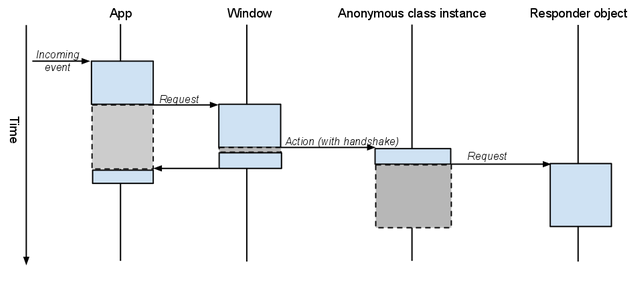
\includegraphics[width=\textwidth]{eventChain.png}
\end{figure}

For window events there is no default responder object, which means that unless a custom responder has been installed, the event will not propagate further then to the anonymous object. However, for input events there is a default input responder, which treats the events differently depending on the type. In case of a key event, the responder method will do the following:
\begin{itemize}
\item the key event is first sent to the currently focused component which is allowed to consume it;
\item if the event is not consumed, the type of key event is inspected; if the event is a key pressed event and the key is Tab, we will try to shift focus forward to the next focusable component in the focus hierarchy.
\end{itemize}
\noindent If the event is a mouse event, this will happen:
\begin{itemize}
\item the responder will iterate through all children of the root container ordered by the time they were added to the container (with the latest addition first), allowing each component that covers the point of the event to consume it until some component has done so;
\item if the component that consumed the event is focusable, the current focus will be shifted to that component.
\end{itemize}

\subsection{Tutorials}

For more information about how to use this interface, please see the tutorial series which covers creating a simple application, adding components into a hierarchy, installing event responders, and opening multiple windows.

\section{Summary}
The following is a list of what has been accomplished in our implementation:
\begin{itemize}
\item a general design of the interface, including the division into modules, the types and the type hierarchy, has been developed;
\item some most important classes from the Cocoa library have been implemented:
\begin{itemize}
\item Window
\item Container
\item Button (at the moment, we cannot set the height of a button)
\item Label
\item Text field
\item Scrollable text area
\item Dropdown list
\end{itemize}
\item an event dispatching mechanism and a focus hierarchy have been implemented.
\end{itemize}

Since this project was limited in time, we focused the time we had for implementation on making sure to include components that would allow us to determine scalability and reliability of our design. Many components had to be omitted, but the set of components we have included are considered sufficient as a foundation for establishing our proof of concept.

Possible improvements that can be made in the future include:
\begin{itemize}
\item implementing customization of application settings (such as adding a dock icon), and the possibility to configure the application menu;
\item delivering key events (key equivalents) to the application's menu;
\item implement some important missing classes, such as canvas and image containers;
\item adding support for the remaining types of mouse events.
\end{itemize}

\subsection{Evaluation}
Our demo apps have shown to work quite well, with performance that is definitely good enough. We can keep a fair amount of objects on the screen and still capture events without any noticeable lag.

One bottleneck we have discovered is that if you place a huge amount of GUI components in a window, the event dispatching will start causing some delays since it loops through all the children to find the destined component. Except for this issue, the applications we have written for testing have worked well.

\section{Experience}
\textit{How we worked}\\
Most of the time we have worked together, with weekly meetings with our supervisor (Andrey Kruglyak). The work started out with a big research process where we learned about the Timber run-time system (rtsPOSIX), Cocoa and garbage collection in general until we had enough knowledge to start designing the interface. The next phase consisted of solving the first design issues, starting with how to combine the run-time systems, the heaps and the GCs. Then came designing the types and the type hierarchy, followed by a lot of implementation. After the implementation phase, in parallel with a lot of testing and final adjustments, we wrote the tutorial series and created the demo applications.
\\ \\ \textit{What we have learned}\\
We have learned a lot in many different areas, including garbage collection in general, the Timber compiler and the Timber run-time system, how GUI libraries work, functional languages and system design. But the most valuable experience has been that we constantly focused not only on finding a workable solution, but on understanding and weighing all the pros and cons of different solutions against each other, in order to reach the solution most suitable for our project. Another important lesson has been that even though you spend a lot of time on designing your project, the implementation phase always takes a lot of time. 
\\ \\ \textit{Reflections}\\
The overall structure with weekly project meetings and performing most of the work together as a group has proven to be a quite effective way to work. The ability to get quick response and feedback from the developers of Timber has also been of tremendous help.

The only big decision we feel we would change, had we taken this course all over again, is not to read it at a reduced rate (we worked for a year at 25\% of time on top of other courses, instead of during half a year at 50\% of time). Even though doing the project over a full year has allowed us to think twice before making decisions, working for this long has resulted in way too much time spent on catching up on things we did earlier, since the work load from other courses made it so that there often had to be multiple days between work sessions.

\newpage
\section{Appendix - CocoaDef.t}
\timbercode{cocoaDef}{}
\begin{thebibliography}{9}
\bibitem{timberLang} \url{http://www.timber-lang.org/}
\bibitem{cocoaLib} \url{http://developer.apple.com/technologies/mac/cocoa.html}
\bibitem{kero1}
 Martin Kero, Johan Nordlander, and Per Lindgren
 \emph{A Correct and Useful Incremental Copying Garbage Collector. In IEEE International Symposium on Memory Management (ISMM)},
 Montreal, QB, 
 2007.
\bibitem{kero2} 
  Martin Kero,
   \emph{Garbage Collection for Reactive Real-Time Systems}, 
  Doctoral thesis, Luleå University of Technology, 
  October 2010

\bibitem{objcRuntime} \url{http://developer.apple.com/library/mac/#documentation/Cocoa/Conceptual/ObjCRuntimeGuide/Introduction/Introduction.html}
\bibitem{cocoaGuidelines} \url{http://developer.apple.com/library/mac/#documentation/UserExperience/Conceptual/AppleHIGuidelines/Intro/Intro.html}
\bibitem{cocoaMemory} \url{http://developer.apple.com/library/mac/#documentation/Cocoa/Conceptual/MemoryMgmt/Articles/mmRules.html}
\bibitem{llvmARC} \url{http://clang.llvm.org/docs/AutomaticReferenceCounting.html}
\bibitem{cocoaGCD} \url{http://developer.apple.com/library/mac/#documentation/Performance/Reference/GCD_libdispatch_Ref/Reference/reference.html}
\bibitem{gcdMainQueue}\url{http://developer.apple.com/library/mac/#documentation/Darwin/Reference/ManPages/man3/dispatch_get_main_queue.3.html}
\bibitem{arcIOS} \url{http://developer.apple.com/library/ios/#releasenotes/General/WhatsNewIniPhoneOS/Articles/iOS5.html#/apple_ref/doc/uid/TP30915195-SW1}
\bibitem{javaFinalize}\url{http://docs.oracle.com/javase/1.4.2/docs/api/java/lang/Object.html}
\end{thebibliography}
\end{document}


